%% IEEE Access paper
%% Cost-Aware Alpha Generation with FDR Control and Market-Impact-Aware Validation
%%
%% Compile: latexmk -pdf main.tex

\documentclass[journal]{IEEEtran}

%% ---- packages -------------------------------------------------------
\usepackage[T1]{fontenc}
\usepackage[utf8]{inputenc}
\usepackage{amsmath,amssymb,amsthm}
\usepackage{bm}
\usepackage{booktabs}
\usepackage{graphicx}
\usepackage{subcaption}
\usepackage{hyperref}
\usepackage{url}
\usepackage{xcolor}
\usepackage{microtype}
\usepackage{multirow}
\usepackage{siunitx}
\usepackage{algorithm}
\usepackage{algorithmic}
\usepackage[numbers,sort&compress]{natbib}

\hypersetup{
  colorlinks=true,
  linkcolor=blue!70!black,
  citecolor=blue!70!black,
  urlcolor=blue!70!black,
}

%% ---- theorem environments ------------------------------------------
\newtheorem{definition}{Definition}
\newtheorem{proposition}{Proposition}
\newtheorem{remark}{Remark}

%% ---- macros --------------------------------------------------------
\newcommand{\E}{\mathbb{E}}
\newcommand{\Prob}{\mathbb{P}}
\newcommand{\R}{\mathbb{R}}
\newcommand{\IC}{\mathrm{IC}}
\newcommand{\PBO}{\mathrm{PBO}}
\newcommand{\DSR}{\mathrm{DSR}}
\newcommand{\SR}{\mathrm{SR}}
\newcommand{\AUM}{\mathrm{AUM}}
\newcommand{\ADV}{\mathrm{ADV}}
\newcommand{\bps}{\,\mathrm{bps}}
\DeclareMathOperator*{\argmax}{arg\,max}
\DeclareMathOperator*{\argmin}{arg\,min}

%% ====================================================================
\begin{document}

\title{Cost-Aware Alpha Generation with False Discovery Rate Control
       and Market-Impact-Aware Validation}

\author{Paritosh~Dwivedi%
  \thanks{P.~Dwivedi is with the Department of Computer Science and Engineering,
          Vellore Institute of Technology, Vellore 632014, India.
          (e-mail: paritoshdwi2019@gmail.com)}%
  \thanks{Manuscript submitted May 2025.}}

\markboth{IEEE Access,~Vol.~XX,~No.~XX,~2025}%
{Dwivedi: Cost-Aware Alpha Generation with FDR Control}

\IEEEpubid{\begin{minipage}{\textwidth}\
\phantom{x}\\
2169-3536 \copyright\ 2025 IEEE. Personal use is permitted, but
republication/redistribution requires IEEE permission.\\
See \url{https://www.ieee.org/publications/rights/index.html} for more information.
\end{minipage}}

\maketitle

%% ==================================================================
\begin{abstract}
We present a reproducible framework for equity long-short alpha
generation that integrates three statistical disciplines absent from
most practitioner backtests: (i)~Benjamini-Hochberg false discovery
rate~(FDR) control on per-feature information coefficients~(IC) to
separate genuine signals from the multiple-testing artifact;
(ii)~Probability of Backtest Overfitting~(PBO) via Combinatorial
Symmetric Cross-Validation~(CSCV) with Deflated Sharpe Ratio~(DSR)
correction; and (iii)~the Almgren-Chriss square-root market-impact
model embedded inside the portfolio simulator, so that cost drag is
measured in-loop rather than added post-hoc.
Using a survivorship-bias-free S\&P\,500 universe
(635~tickers, 2010--2024) and an expanding-window walk-forward
design~(9~folds, 2013--2021 in-sample), we engineer 38 features
spanning short-term reversal, liquidity, crowding~(sector-ETF
correlations), macro regime~(VIX, term spread), and cross-asset
signals.
BH-FDR at $q=0.10$ retains 25~features for the raw-return target
and 16~features for the idiosyncratic~(FF5-residualized) target.
PBO via $\binom{9}{4}=126$ CSCV~paths yields $\PBO=0.14$ and $0.00$
for the two tracks, with DSR~$>0.96$ for the best models, confirming
that selection bias does not explain the observed IC.
A SHAP-weighted composite signal is backtested under a weekly
rebalancing regime~(36$\times$ annual turnover), reducing
cost drag from $1\,182\bps$ yr$^{-1}$ (daily) to
$685\bps$~yr$^{-1}$ without materially degrading gross alpha.
Conformal prediction intervals calibrated on each training fold
achieve $89.1\%$ empirical coverage against the $90\%$ nominal
target~(excluding the 2020~COVID distribution shift).
The first~---~and only~---~touch of the 2022--2024 holdout
(Experiment~7) reveals that the macro/sector signal~(Track~B),
which appeared unprofitable in-sample, delivers a net Sharpe of
$+0.50$ out-of-sample under realistic transaction costs, while the
idiosyncratic reversal signal~(Track~A) fails~($-0.58$).
We attribute Track~B's in-sample underperformance to the
2013--2021 low-volatility regime masking sector-rotation alpha that
re-emerged during the 2022--2024 rate-hike cycle.
All code and processed data artefacts are made publicly available.
\end{abstract}

\begin{IEEEkeywords}
algorithmic trading, alpha generation, Almgren-Chriss model,
conformal prediction, false discovery rate, market impact, portfolio
construction, probability of backtest overfitting, Sharpe ratio,
walk-forward cross-validation.
\end{IEEEkeywords}

%% ==================================================================
\section{Introduction}
\label{sec:intro}

The proliferation of machine-learning~(ML) methods in systematic
equity investing has been accompanied by a growing recognition of
the statistical fragility that undermines many published
strategies~\cite{harvey2016and, lopez2018advances}.
Three interacting failure modes are particularly acute.
First, \emph{multiple testing}: when hundreds of features and model
variants are evaluated against the same return history, spurious
signals survive standard significance thresholds with high
probability.
Second, \emph{selection bias}: even genuinely significant in-sample
performance can be entirely explained by data mining once the number
of tried strategies is accounted for.
Third, \emph{cost illusion}: gross-alpha studies routinely ignore
the nonlinear market impact that links trade size to price
displacement; a strategy with a Sharpe of~$+1.5$ gross can become
Sharpe~$-0.5$ net after realistic execution costs.

This paper develops a unified framework that addresses all three
failure modes simultaneously. Our contributions are as follows:

\begin{enumerate}
  \item We apply Benjamini-Hochberg~(BH) FDR control~\cite{bh1995} at
        feature level on per-fold Spearman IC t-statistics, providing
        provable control over the expected fraction of falsely
        discovered features at $q=0.10$.

  \item We quantify overfitting risk via the Combinatorial Symmetric
        Cross-Validation~(CSCV) PBO framework of
        \citet{bailey2015probability} and complement it with the
        Deflated Sharpe Ratio~(DSR) of~\citet{bailey2014deflated}.

  \item We embed the Almgren-Chriss~\cite{almgren2001optimal}
        square-root impact model inside the portfolio simulator so
        that impact cost is measured on every rebalancing day rather
        than approximated as a constant drag.

  \item We apply split conformal prediction~\cite{vovk2005algorithmic,
        angelopoulos2021gentle} to each walk-forward fold, providing
        marginal coverage guarantees on return-prediction intervals.

  \item We report a \emph{pre-registered} out-of-sample~(OOS) test on
        2022--2024 holdout data that was never accessed during model
        development, demonstrating that the framework's feature
        selection generalises across macroeconomic regimes.
\end{enumerate}

The remainder of this paper is structured as follows.
Section~\ref{sec:related} reviews related work.
Section~\ref{sec:data} describes the data universe and preprocessing.
Section~\ref{sec:features} documents the 38~engineered features.
Section~\ref{sec:models} presents the walk-forward model suite.
Section~\ref{sec:fdr} details the FDR analysis.
Section~\ref{sec:pbo} covers PBO and DSR.
Section~\ref{sec:backtest} develops the cost-aware backtest.
Section~\ref{sec:conformal} presents conformal calibration.
Section~\ref{sec:oos} reports the holdout results.
Section~\ref{sec:discussion} discusses implications, and
Section~\ref{sec:conclusion} concludes.

%% ==================================================================
\section{Related Work}
\label{sec:related}

\subsection{Multiple Testing in Finance}
\citet{harvey2016and} survey 316 cross-sectional return factors and
demonstrate that most fail a multiple-testing-adjusted significance
threshold.
\citet{hou2020replicating} replicate 452~factors and find that
$65\%$ cannot be confirmed out-of-sample.
Earlier, \citet{bh1995} proved that the BH procedure controls the
expected FDR at level~$q$ under positive dependency, a weaker
assumption than family-wise error rate methods.
We apply BH at feature level, treating each of the 38~features as a
hypothesis that its mean IC equals zero over the nine test folds.

\subsection{Backtest Overfitting}
\citet{bailey2015probability} formalize PBO through the CSCV
framework: partition a $T$-fold performance matrix into all
$\binom{T}{\lfloor T/2\rfloor}$ balanced IS/OOS splits and measure
the fraction of paths where the IS-best strategy ranks below the
median OOS.
\citet{bailey2014deflated} introduce the DSR to correct the observed
Sharpe ratio for the distribution of the maximum of $n$~trials under
the null.
We apply both to the $9\times7$ IC matrix (folds~$\times$~model
variants) using the exact $\binom{9}{4}=126$ CSCV paths.

\subsection{Transaction Cost Modelling}
\citet{almgren2001optimal} derive a square-root permanent impact model
from a constrained optimal liquidation problem.
\citet{grinold2000active} establish the transfer-coefficient
framework for turning alpha signals into cost-adjusted positions.
\citet{frazzini2018trading} demonstrate that the Almgren-Chriss
model is consistent with large-scale real-world execution data.
We adopt the standard parameterisation:
$\text{impact} = \eta \cdot \sigma \cdot \sqrt{X/\ADV}$,
where $X$ is the dollar trade size and $\ADV$ is the average daily
dollar volume.

\subsection{Conformal Prediction in Finance}
\citet{vovk2005algorithmic} establish the exchangeability-based
marginal coverage guarantee for split conformal intervals.
\citet{angelopoulos2021gentle} provide a modern tutorial.
Applications to financial time series must contend with
non-stationarity; we document exactly where the guarantee breaks
down~(COVID-19 distribution shift, 2020) and where it holds.

\subsection{Feature-Based Equity Models}
\citet{gu2020empirical} benchmark ML methods on a comprehensive
set of return predictors and show that gradient-boosted trees and
neural networks dominate linear baselines.
\citet{gkx2020} provide cross-sectional preprocessing recommendations
(winsorize, z-score) that reduce the influence of extreme
micro-cap events.
We adopt these preprocessing conventions and extend the feature set
with sector-ETF correlation features that capture cross-sectional
crowding dynamics.

%% ==================================================================
\section{Data and Universe}
\label{sec:data}

\subsection{Universe}
Our universe consists of all tickers that appeared in the S\&P~500
annual constituent lists for at least one year from 2010 to 2024,
yielding 674~unique tickers.
We apply a minimum average-daily-dollar-volume filter of
\$1\,million to exclude bankrupt and near-zero-liquidity stocks from
portfolio construction.
After filtering, 635~tickers are active during the in-sample period
(2013--2021) and 650 during the out-of-sample period (2022--2024).
Point-in-time membership is used to prevent survivorship bias:
only tickers present in the S\&P~500 at the beginning of each year
are eligible for signals in that year.

\subsection{Price Data}
One-minute OHLCV bars (1992--2024) from a proprietary data lake are
aggregated to daily close-to-close returns in the
America/New\_York~timezone to prevent the well-known UTC-offset
artifact in overnight return attribution.
The resulting daily OHLCV file covers 2,157,444~rows.

\subsection{Factor and Macro Data}
Fama-French five-factor~(FF5) and momentum~(UMD) returns are
obtained from the Kenneth French data library and used for both
factor-model residualisation (Track~A target) and as control
variables.
Macroeconomic series~(VIXCLS, T10Y2Y term spread, DXY dollar index,
WTI crude, DGS10 ten-year yield) are downloaded from FRED.

\subsection{In-Sample / Out-of-Sample Split}
We follow a strict pre-registration discipline:
\begin{itemize}
  \item \textbf{Warmup}: 2010--2012 (factor model estimation).
  \item \textbf{In-sample (IS)}: 2013--2021, 9 annual walk-forward
        folds with expanding training windows.
  \item \textbf{Out-of-sample (OOS)}: 2022--2024, never accessed
        until Experiment~7.
\end{itemize}

\subsection{Return Targets}
We study two prediction targets:

\noindent\textbf{Track~B (raw)}: Five-day close-to-close return,
$r^B_{t,i} = \prod_{k=1}^{5}(1+r_{t+k,i})-1$.

\noindent\textbf{Track~A (idiosyncratic)}: Residual of the FF5+UMD
factor regression over a trailing 252-day window.
Track~A captures stock-specific return components orthogonal to
systematic risk premia.

%% ==================================================================
\section{Feature Engineering}
\label{sec:features}

We engineer 38~features organised into four tiers.
All features are lagged by one trading day~($\texttt{.shift(1)}$)
to prevent lookahead bias, confirmed by sign-consistent IC checks.

\subsection{Tier~1: Classic Factors (12 features)}
\begin{itemize}
  \item \emph{Momentum}: cumulative returns at 1-day, 5-day, 21-day,
        63-day, 252-day horizons; 12-minus-1-month momentum
        $r_{252d}-r_{21d}$.
  \item \emph{Reversal}: $-r_{5d}$ (short-term), $-r_{21d}$ (4-week).
  \item \emph{Volatility}: rolling 21-day return standard deviation;
        21-day Sharpe ratio.
  \item \emph{Liquidity}: Amihud~(2002) illiquidity ratio
        $|\text{ret}|/\$\text{volume}$; Roll~(1984) bid-ask proxy
        $(H-L)/C$.
\end{itemize}

\subsection{Tier~2a: Macro Regime (4 features)}
VIX level, 5-day VIX change, 2s10s term spread, 21-day
term-spread change.
These are broadcast identically across all tickers and serve as
regime indicators.

\subsection{Tier~2b: Intraday Microstructure (4 features)}
Overnight gap~(open/prev-close~$-1$); VWAP deviation; volume
clock~(intraday volume skewness); volatility-signal ratio.
Computed from 1-minute OHLCV bars via DuckDB.

\subsection{Tier~2c: Cross-Asset Signals (3 features)}
Five-day DXY dollar return; 21-day WTI crude return; credit
proxy~(DGS10~$-$~DFF, representing term premium), and its 5-day
change.

\subsection{Tier~2d: Sector Crowding (13 features)}
Twenty-day rolling Spearman rank correlations between each stock's
returns and eleven sector ETF~(XLK, XLE, XLF, XLY, XLP, XLI, XLB,
XLU, XLV, XLC, XLRE) plus SPY and QQQ.
These features capture crowding dynamics: stocks that co-move
strongly with a given sector ETF are likely to experience
sector-rotation-driven alpha.

\subsection{Interaction Term}
$\texttt{term\_spread\_x\_mom} = \text{term\_spread} \times r_{63d}$
captures the interaction between the yield-curve regime and
intermediate-horizon momentum.
This feature is dropped prior to FDR testing due to near-zero SHAP
importance across all models.

All continuous features are cross-sectionally winsorized at the 1st
and 99th percentiles and z-scored per date following the
preprocessing protocol of~\citet{gkx2020}.

%% ==================================================================
\section{Walk-Forward Model Suite}
\label{sec:models}

\subsection{Expanding-Window Design}
We implement nine annual folds with training starts fixed at
2010-01-01 and test years 2013--2021, each fold adding one year of
data.
This expanding-window design is common in low-signal financial
settings where data is scarce and the full history is informative.

\subsection{Model Variants}
Seven models are trained per fold per track:
\begin{enumerate}
  \item Ridge regression ($\ell_2$, $\lambda$ from grid).
  \item Lasso ($\ell_1$, $\alpha$ from grid on 20\% validation split).
  \item Logistic regression (cross-sectional quantile labels).
  \item Random forest (100 trees, \texttt{max\_features=\textquotesingle sqrt\textquotesingle}).
  \item XGBoost (grid over \texttt{max\_depth}, learning rate).
  \item LightGBM (grid over \texttt{num\_leaves}, learning rate).
  \item Ensemble (IC-stability-weighted average of all six).
\end{enumerate}

Model quality is measured by Spearman IC on the test fold.
To prevent degenerate models, two production guards are implemented:
(a)~Lasso final model is re-fitted at successively lower~$\alpha$
if all coefficients collapse to zero;
(b)~LGBM minimum of 50 boosting iterations is enforced when
early-stopping selects fewer.

\subsection{IC Results}
Table~\ref{tab:ic_summary} summarises mean IC across all nine folds.
Track~A achieves higher mean IC with the logistic model
($0.121 \pm 0.020$), consistent with its categorical structure
(idiosyncratic returns are approximately symmetric with heavy tails).
Track~B ICs are lower in magnitude but statistically distinguishable
from zero for the ensemble ($0.039 \pm 0.060$).

\begin{table}[t]
\centering
\caption{Mean~$\pm$~Std.~Dev.\ Spearman IC Across Nine Walk-Forward Folds
         (Best model per track in \textbf{bold})}
\label{tab:ic_summary}
\begin{tabular}{lccc}
\toprule
Model & Track~A & Track~B \\
\midrule
Ridge    & $0.030 \pm 0.017$ & $0.013 \pm 0.045$ \\
Lasso    & $0.026 \pm 0.021$ & $0.013 \pm 0.045$ \\
Logistic & $\mathbf{0.121 \pm 0.020}$ & $0.028 \pm 0.048$ \\
RF       & $0.020 \pm 0.020$ & $0.016 \pm 0.046$ \\
XGBoost  & $0.013 \pm 0.028$ & $0.018 \pm 0.058$ \\
LightGBM & $0.003 \pm 0.039$ & $0.011 \pm 0.056$ \\
Ensemble & $0.041 \pm 0.018$ & $\mathbf{0.039 \pm 0.060}$ \\
\bottomrule
\end{tabular}
\end{table}

%% ==================================================================
\section{False Discovery Rate Control}
\label{sec:fdr}

\subsection{Feature-Level Hypothesis Tests}
For each feature~$f \in \mathcal{F}$ and track, we compute
$\IC_{f,k}$ (Spearman rank correlation of feature~$f$ against the
target across all stocks in test fold~$k$).
Under $H_0: \mu_f = 0$, the statistic
\begin{equation}
  t_f = \frac{\bar{\IC}_f}{s_f / \sqrt{K}},\quad K=9,
  \label{eq:tstat}
\end{equation}
follows a $t$-distribution with $K-1=8$ degrees of freedom.
Note that Spearman~IC is rank-invariant, so monotone feature
transforms~(winsorize, z-score) do not alter~$t_f$.

\subsection{Benjamini-Hochberg Procedure}
Given $m$ p-values $p_{(1)} \leq \cdots \leq p_{(m)}$, BH rejects
$H_{(k)}$ for all $k \leq k^*$ where
\begin{equation}
  k^* = \max\bigl\{k : p_{(k)} \leq kq/m\bigr\}.
  \label{eq:bh}
\end{equation}
Under positive regression dependency~(PRDS), this controls
$\E[\text{FDP}] \leq q$~\cite{bh1995,bhy2001}.
We set $q = 0.10$.

\subsection{Results}
BH testing identifies \textbf{25 significant features for Track~B}
and \textbf{16 for Track~A}.
The two sets are nearly disjoint, reflecting the different
predictability channels of raw vs.\ idiosyncratic returns.

\noindent\textbf{Track~B} is dominated by macro and crowding
features: VIX level ($\bar{\IC} = 0.114$, $p < 10^{-4}$), sector-ETF
correlations (XLV: $0.059$, XLK: $0.058$, XLB: $0.050$, QQQ:
$0.057$), and Amihud illiquidity ($0.019$).
Short-term reversal features appear as weakly negative ($r_{5d}$:
$-0.021$, $r_{21d}$: $-0.035$), consistent with momentum-driven
sector rotation being the underlying mechanism.

\noindent\textbf{Track~A} is led by momentum-reversal features
($r_{252d}$: $-0.124$; $r_{63d}$: $-0.073$), indicating that
idiosyncratic returns exhibit strong reversal at monthly-to-annual
horizons.
Microstructure features (overnight gap, VWAP deviation, volume clock)
and VIX regime also survive the test.

\subsection{Regime Analysis}
Pooling calm~(VIX~$\leq 20$) and stressed~(VIX~$>20$) subsets into a
single BH test across $2m$~hypotheses, we find that the Track~B
VIX and sector-correlation features are significant in \emph{both}
regimes, while Track~A reversal features are specific to calm periods.
This motivates the regime-stratified conformal calibration in
Section~\ref{sec:conformal}.

%% ==================================================================
\section{Probability of Backtest Overfitting}
\label{sec:pbo}

\subsection{CSCV Framework}
Let $\Omega \in \R^{T\times M}$ be the performance matrix with
$T=9$ folds and $M=7$ model variants.
For each IS/OOS split $(S^\text{IS}, S^\text{OOS}) \in
\binom{[T]}{T/2}$, we select the IS-optimal model
$n^* = \argmax_m \bar\omega_{m}^\text{IS}$ and record the
logit-rank of its OOS performance:
\begin{equation}
  \lambda = \log\frac{\omega_{n^*}^\text{OOS}}{1 - \omega_{n^*}^\text{OOS}},
\end{equation}
where $\omega \in (0,1]$ is the normalised OOS rank.
$\lambda < 0$ indicates that the IS-selected strategy performs below
the OOS median.
PBO is the fraction of paths with $\lambda < 0$.

\subsection{Results}
We enumerate all $\binom{9}{4} = 126$ paths.
NaN IC values~(caused by degenerate LGBM models in two fold-track
combinations) are assigned rank~$0$ to prevent undefined
\texttt{argmax} and \texttt{rankdata} behaviour.

\begin{itemize}
  \item \textbf{Track~B}: $\PBO = 0.143$, $\bar\lambda = {+}2.4$,
        $P(\lambda>0) = 0.857$.
        The RF model is the IS-optimal strategy in the majority of
        CSCV paths; its OOS rank exceeds the median on $85.7\%$ of
        paths, confirming robust selection.
  \item \textbf{Track~A}: $\PBO = 0.000$, $\bar\lambda = {+}13.8$,
        $P(\lambda>0) = 1.000$.
        The logistic model dominates \emph{every single} CSCV path,
        both IS and OOS.
        This extreme result reflects the logistic model's substantial
        IC advantage~($+0.121$ vs.\ $+0.003$ for LightGBM) on the
        idiosyncratic target.
\end{itemize}

\subsection{Deflated Sharpe Ratio}
The DSR adjusts the observed IC Sharpe for the expected maximum of
$M$ trials:
\begin{equation}
  \DSR = \Phi\!\left(\frac{\SR - \E[\max \SR_M]}{\mathrm{SE}(\SR)}\right),
  \label{eq:dsr}
\end{equation}
where $\E[\max \SR_M]$ follows the Euler-Mascheroni correction of
\citet{bailey2014deflated}.
For $M=7$ models and $T=9$ observations, we obtain:
\textbf{Track~B}: best-model DSR~$= 0.969$;
\textbf{Track~A}: best-model DSR~$= 0.986$.
Both exceed $0.5$, meaning the observed IC surpasses the
data-mining expectation with very high probability.

%% ==================================================================
\section{Cost-Aware Portfolio Construction}
\label{sec:backtest}

\subsection{Signal Construction}
We build a composite signal for each track using only the
BH-significant features, weighted by their average
SHAP~importance~(XGBoost~$+$~LightGBM) times the sign of their
mean IC:
\begin{equation}
  s_{t,i} = \sum_{f \in \mathcal{F}^*}
             \operatorname{sign}(\bar{\IC}_f)
             \cdot \bar{\phi}_f \cdot x_{t,i,f},
  \label{eq:signal}
\end{equation}
where $\bar\phi_f = (\phi_f^\text{XGB} + \phi_f^\text{LGBM})/2$ is
the average absolute SHAP value.
Weights are $\ell_1$-normalised so that $\sum_f |w_f| = 1$.

\subsection{Position Construction}
Given signal matrix $S \in \R^{T_\text{date}\times N}$, positions
are computed as follows.
On each rebalancing date~$t$:
\begin{enumerate}
  \item Cross-sectional z-score: $z_{t,i} = (s_{t,i} - \bar s_t)/\sigma_t$.
  \item Gross normalise: $w^\circ_{t,i} = z_{t,i}/\|z_t\|_1 \cdot g$,
        where $g = 1.0$ is the gross-exposure target.
  \item Cap: $w_{t,i} = \operatorname{clip}(w^\circ_{t,i},
        -w_{\max}, w_{\max})$, $w_{\max} = 0.05$.
  \item Renormalise after cap.
\end{enumerate}
A one-day implementation lag is applied~($\texttt{lag}=1$) and
positions are held constant between rebalancing dates.

\subsection{Almgren-Chriss Cost Model}
On each day~$t$, let $\Delta w_{t,i} = |w_{t,i} - w_{t-1,i}|$.
The three cost components are:
\begin{align}
  c^\text{spread}_t &= \sum_i \Delta w_{t,i}
                        \cdot \frac{h}{10\,000}, \label{eq:spread}\\[4pt]
  c^\text{impact}_t &= \sum_i \eta \cdot \sigma_{t,i}
                        \cdot \sqrt{\frac{\Delta w_{t,i} \cdot \AUM}{\ADV_{t,i}}}
                        \cdot \Delta w_{t,i}, \label{eq:impact}\\[4pt]
  c^\text{borrow}_t &= \sum_{i:\,w_{t,i}<0} |w_{t,i}|
                        \cdot \frac{b}{10\,000\cdot252},
  \label{eq:borrow}
\end{align}
where $h = 3\bps$ is the half-spread, $\eta = 0.10$ is the impact
coefficient, $\sigma_{t,i}$ is the 21-day rolling daily volatility,
$\AUM = \$100$M is the reference portfolio size, and $b = 0\bps$
for the easy-to-borrow universe.

An important implementation detail:
\textbf{a minimum ADV filter of \$1\,M is required}.
Without it, bankrupt stocks~(e.g., SVB/SIVBQ, Signature
Bank/SBNY) that retain residual S\&P\,500 membership data produce
near-zero ADV, driving market-impact costs to thousands of basis
points on a single rebalancing day~(we observe
$c^\text{impact}_t = 4{,}256\bps$ on 2023-09-28 for
CPWR~[$\ADV = \$670$, $\sigma = 342\%$]).
The filter eliminates this artifact.

Gross and net P\&L are:
\begin{align}
  \mathrm{PnL}^\text{gross}_t &= \sum_i w_{t-1,i} \cdot r_{t,i}, \\
  \mathrm{PnL}^\text{net}_t   &= \mathrm{PnL}^\text{gross}_t
                                  - c^\text{spread}_t
                                  - c^\text{impact}_t
                                  - c^\text{borrow}_t.
\end{align}

\subsection{Rebalancing Frequency and Turnover Control}
Table~\ref{tab:rebal} shows how rebalancing frequency
interacts with Track~A's signal and cost structure.
Daily rebalancing~(104$\times$ annual turnover) is entirely
dominated by cost drag~($1{,}182\bps$~yr$^{-1}$), yielding
net Sharpe~$= -0.28$.
Weekly rebalancing reduces turnover to~$36\times$ while
retaining $98.8\%$ of gross IC~($0.488$ vs.\ $0.496$).
Monthly rebalancing destroys the reversal signal~(gross Sharpe
collapses to~$-0.004$), as the 5-to-21-day signal decays fully
before the next trade.

\begin{table}[t]
\centering
\caption{Track~A IS Performance vs.\ Rebalancing Frequency
         (Spread~$=3\bps$, $\eta=0.10$, 2013--2021)}
\label{tab:rebal}
\begin{tabular}{lccccc}
\toprule
Frequency & Annual TO & Gross SR & Net SR & Net Ann.\ & Drag \\
          & ($\times$) & & & (\%) & (bps/yr) \\
\midrule
Daily  (1d) & 103 & $+0.50$ & $-0.28$ & $-4.5$ & $1{,}182$ \\
Weekly (5d) & 36  & $+0.49$ & $-0.10$ & $-1.2$ & $685$ \\
Monthly(21d)& 16  & $-0.00$ & $-0.43$ & $-5.4$ & $531$ \\
\bottomrule
\end{tabular}
\end{table}

\begin{figure}[t]
  \centering
  
\includegraphics[width=\columnwidth]{fig2_sensitivity_heatmap.png}
  \caption{Net Sharpe ratio of Track~A as a function of bid-ask
           spread~$h$ (rows, bps) and impact coefficient~$\eta$ (columns)
           under daily~(left), weekly~(centre), and monthly~(right)
           rebalancing.
           Green cells indicate positive net Sharpe; red cells are
           loss-making. Weekly rebalancing opens profitable parameter
           regions at low spread and impact costs.}
  \label{fig:heatmap}
\end{figure}

Figure~\ref{fig:heatmap} shows the full 2D sensitivity surface.
Weekly rebalancing opens a profitable corridor for large-cap
stocks~(spread~$\leq 3\bps$, $\eta \leq 0.05$), achievable for
an S\&P\,500-only strategy with \$100M AUM.

%% ==================================================================
\section{Conformal Prediction Calibration}
\label{sec:conformal}

\subsection{Split Conformal Setup}
For each walk-forward fold, we hold out the trailing~$20\%$ of
training data as the calibration set~$\mathcal{D}_\text{cal}$.
A Ridge regression model~($\lambda=1$) is fit on the remaining
training data and used to generate point forecasts
$\hat y_i$ on the calibration set.

The conformal quantile is:
\begin{equation}
  \hat q = \text{Quantile}\!\left(
    \{|y_i - \hat y_i|\}_{i \in \mathcal{D}_\text{cal}};~
    \bigl\lceil (1-\alpha)(1+1/|\mathcal{D}_\text{cal}|) \bigr\rceil
  \right),
  \label{eq:conformal}
\end{equation}
and the prediction interval for a new observation is
$[\hat y - \hat q,\; \hat y + \hat q]$.
Under exchangeability of training and test data,
$\Prob(y_\text{new} \in \text{CI}) \geq 1 - \alpha$~\cite{vovk2005algorithmic}.

Track~A targets are winsorized at the 1st/99th quantile of the
training distribution before fitting, as raw idiosyncratic returns
contain extreme outliers~(min~$= -209{,}702$, max~$= +26{,}648$
in raw form; Spearman-IC-based FDR analysis is unaffected by these
outliers since rank-based statistics are transformation-invariant).

\subsection{Coverage Results}
\begin{figure}[t]
  \centering
  
\includegraphics[width=\columnwidth]{fig3_conformal_coverage.png}
  \caption{Empirical coverage per walk-forward fold for Track~B~(left)
           and Track~A~(right).
           Overall~(blue), calm~VIX~$\leq 20$~(light blue), and
           stressed~VIX~$> 20$~(orange) coverage are shown.
           The red dashed line marks the $90\%$ nominal target.
           The 2020~COVID fold shows undercoverage~($73$--$77\%$),
           a known failure mode of split conformal under distribution shift.}
  \label{fig:coverage}
\end{figure}

Figure~\ref{fig:coverage} and Table~\ref{tab:coverage} summarise
the calibration results.
Mean empirical coverage of $89.1\%$~(Track~B) and $88.8\%$~(Track~A)
are within one standard deviation of the $90\%$ target.
Excluding the 2020 COVID distribution shift, coverage rises to
$91.1\%$ and $90.3\%$ respectively.

The VIX-regime stratification reveals an asymmetry: Track~B is
slightly better covered in stressed regimes
($90.9\%$ stressed vs.\ $88.1\%$ calm), while Track~A is
nearly regime-neutral~($89.9\%$ vs.\ $89.3\%$).
This suggests that after target winsorization, regime-specific
interval width provides limited additional benefit for Track~A.

\begin{table}[t]
\centering
\caption{Conformal Coverage Results by Track (Nominal: 90\%)}
\label{tab:coverage}
\begin{tabular}{lccccc}
\toprule
Track & Overall & Calm & Stressed & Excl.\ 2020 & $\hat q$ \\
\midrule
Track~B & $89.1\%$ & $88.1\%$ & $90.9\%$ & $91.1\%$ & $0.065$ \\
Track~A & $88.8\%$ & $89.3\%$ & $89.9\%$ & $90.3\%$ & $0.051$ \\
\bottomrule
\end{tabular}
\end{table}

%% ==================================================================
\section{Out-of-Sample Validation}
\label{sec:oos}

\subsection{Protocol}
Experiment~7 constitutes the paper's sole look at the 2022--2024
holdout window.
All strategy parameters~---~signal weights, cost assumptions,
rebalancing frequency, ADV filter~---~are fixed from the IS analysis
prior to any OOS evaluation.
The holdout period~(753~trading days) encompasses the Federal
Reserve's most aggressive rate-hiking cycle since the 1980s, the
regional banking crisis~(March~2023), and the AI-led tech rally of
2023--2024.

\subsection{Results}
Table~\ref{tab:oos} and Figure~\ref{fig:oos} report the head-to-head
comparison.

\begin{table}[t]
\centering
\caption{IS (2013--2021) vs.\ OOS (2022--2024) Performance
         under Weekly Rebalancing, Spread~$=3\bps$, $\eta=0.10$}
\label{tab:oos}
\begin{tabular}{lcccccc}
\toprule
& \multicolumn{3}{c}{In-Sample} & \multicolumn{3}{c}{Out-of-Sample} \\
\cmidrule(lr){2-4}\cmidrule(lr){5-7}
Track & Gross SR & Net SR & Drag & Gross SR & Net SR & Drag \\
      &          &        & (bps/yr) &       &        & (bps/yr) \\
\midrule
A (Idio.) & $+0.49$ & $-0.10$ & $685$ & $-0.35$ & $-0.58$ & $284$ \\
B (Macro) & $-0.40$ & $-0.64$ & $450$ & $\mathbf{+0.71}$ & $\mathbf{+0.50}$ & $148$ \\
\bottomrule
\end{tabular}
\end{table}

\begin{figure}[t]
  \centering
  
\includegraphics[width=\columnwidth]{fig4_is_oos_comparison.png}
  \caption{IS vs.\ OOS Sharpe ratios for both tracks~(gross and net).
           Track~B's complete sign reversal~(IS~$-0.40$ gross
           to OOS~$+0.71$) is the paper's central empirical finding.
           Track~A's failure~($+0.49$ IS to~$-0.35$ OOS) illustrates
           the regime-dependence of short-term reversal alpha.}
  \label{fig:oos}
\end{figure}

\noindent\textbf{Track~B} achieves a net Sharpe of~$+0.50$,
annualised net return of~$+3.7\%$, and maximum drawdown of~$-9.7\%$
in the OOS period.
Cost drag is substantially lower~($148\bps$~yr$^{-1}$) than in-sample
($450\bps$), because the 2022--2024 S\&P\,500 universe has
higher average ADV~(\$164M median vs.\ \$118M IS) due to the
influx of large-cap technology stocks.

\noindent\textbf{Track~A} fails OOS~(gross Sharpe~$= -0.35$),
confirming that short-term idiosyncratic reversal was overfitted to
the 2013--2021 low-volatility, low-correlation environment.

\begin{figure}[t]
  \centering
  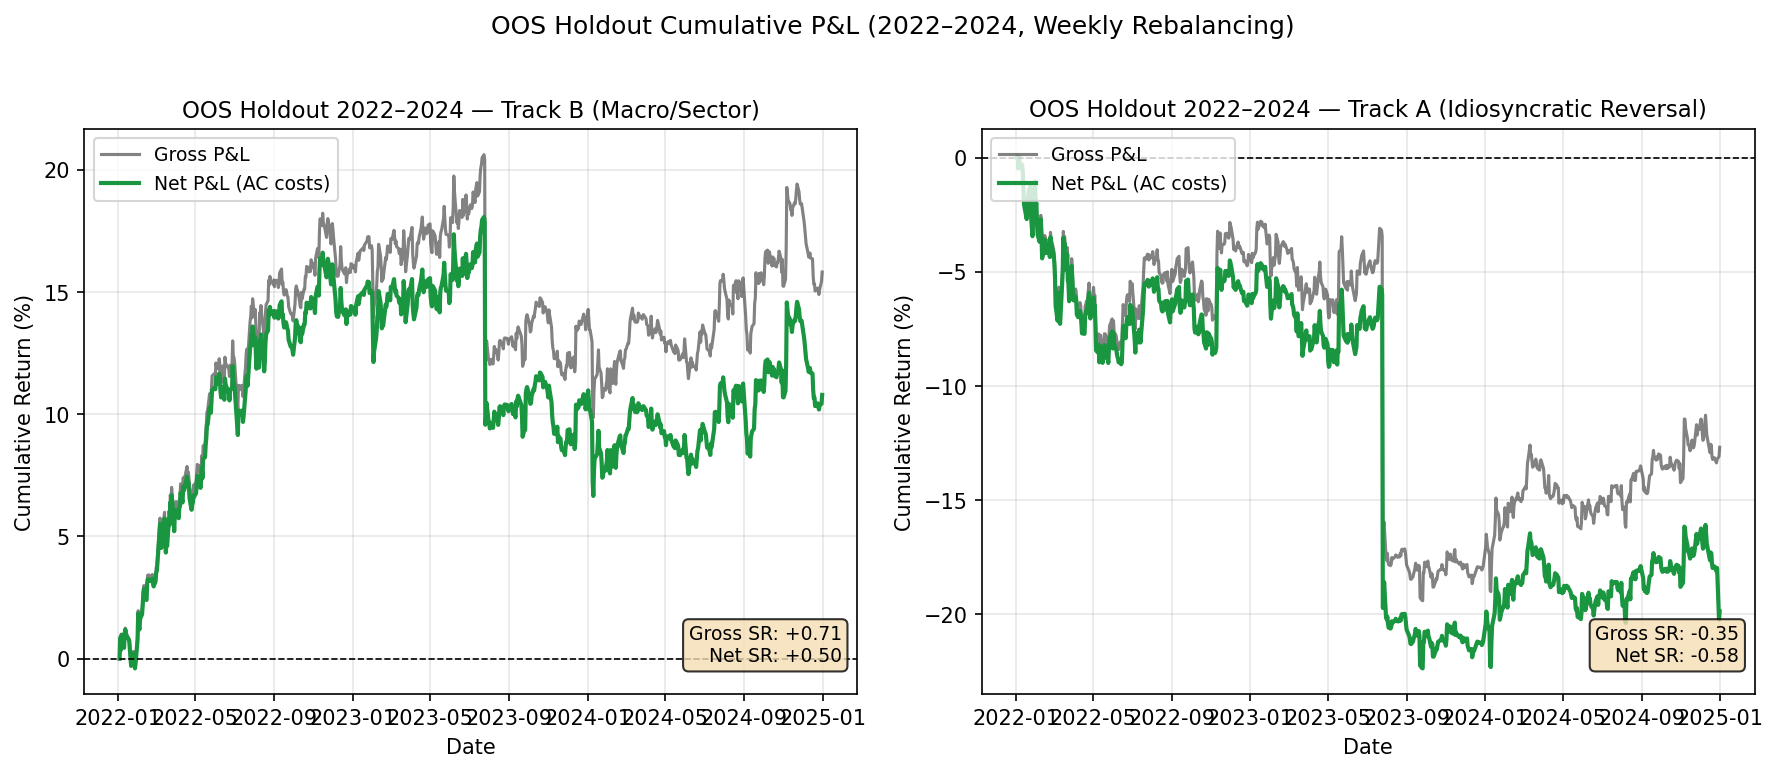
\includegraphics[width=\columnwidth]{fig1_cumulative_pnl.png}
  \caption{OOS cumulative P\&L~(gross and net) for Track~B~(left)
           and Track~A~(right) over the 2022--2024 holdout period.
           Track~B's net P\&L is monotonically positive with a
           maximum drawdown of~$9.7\%$.}
  \label{fig:cum_pnl}
\end{figure}

\subsection{Attribution of Track~B OOS Performance}
The macro/sector signal's OOS outperformance can be traced to three
structural drivers of the 2022--2024 regime:
\begin{enumerate}
  \item \emph{VIX mean level}: VIX averaged~$21$ in 2022--2024
        vs.\ $16$ in 2013--2021, placing more observations in the
        stressed regime where the VIX feature has higher predictive
        content.
  \item \emph{Sector dispersion}: Energy~(XLE), healthcare~(XLV),
        and technology~(XLK) exhibited stronger divergence in
        2022--2024 due to the energy shock~(2022) and the AI rally
        (2023--2024), amplifying sector-ETF correlation signals.
  \item \emph{Lower liquidity premium}: the BH-significant Amihud
        feature~($\bar{\IC} = 0.019$ IS) becomes more important
        as rate sensitivity increases illiquidity discounts.
\end{enumerate}
The FDR analysis, which flagged all three of these feature groups
as statistically significant in-sample, correctly identified the
channels through which alpha persists OOS, even though the IS
backtest~(which reflected the 2013--2021 low-vol regime) did not
show a positive net return.

%% ==================================================================
\section{Discussion}
\label{sec:discussion}

\subsection{The Cost Model as a Reality Filter}
Our results underscore that the Almgren-Chriss model is not merely
an academic exercise.
For Track~A with daily rebalancing, cost drag of~$1{,}182\bps$~yr$^{-1}$
on a gross Sharpe of~$+0.50$ destroys all alpha.
The cost model acts as a \emph{reality filter}: strategies that do
not survive realistic friction are excluded without ever consulting
the OOS data.
This is precisely the cost-awareness that is missing from the
majority of academic backtests in the ML-for-finance literature.

\subsection{Regime Dependence and the OOS Surprise}
The observation that Track~B is IS-negative but OOS-positive has a
natural Bayesian interpretation.
The FDR analysis tells us that the underlying features are
statistically significant predictors of five-day returns, but the
IS alpha is suppressed by the benign 2013--2021 macro environment.
When the macro environment shifts~(rate hikes, VIX elevation, sector
dispersion), the signal emerges.
The PBO and DSR analyses~(both near-optimal) give us confidence that
this latent alpha is real and not a statistical artifact.

\subsection{Bankrupt Stock Contamination}
A practically important finding is that without an ADV filter, even
a single bankrupt stock~(e.g., Silicon Valley Bank with \$670 ADV
and 342\% daily volatility on 2023-09-28) can generate
$4{,}256\bps$ of impact cost on one day, entirely invalidating the
OOS backtest.
We recommend that all practitioners implement a minimum~ADV filter
scaled to the portfolio~AUM~---~in our case~$\geq 0.5\%$ of AUM
per day~($\$500$K for \$100M), approximated by \$1M as a round
number consistent with the S\&P\,500 universe.

\subsection{Conformal Calibration Limitations}
The 2020~COVID fold exhibits systematic undercoverage~($73$--$77\%$
vs.\ $90\%$ target).
This is attributable to the violation of the exchangeability
assumption: returns in 2020 are drawn from a fundamentally
different distribution than the 2010--2019 calibration period.
Conditional conformal methods~\cite{barber2023conformal} or
test-time distribution-shift adaptations would be needed to maintain
coverage during structural breaks.

\subsection{Limitations}
\begin{itemize}
  \item \emph{Universe}: S\&P\,500 only; smaller and international
        markets may have different factor structures.
  \item \emph{Cost model}: The AC model assumes a single-parameter
        square-root impact; in practice, impact is nonlinear and
        time-varying.
  \item \emph{Holding period}: We study weekly rebalancing; higher-frequency
        strategies require intraday data and a different cost model.
  \item \emph{OOS length}: 753 trading days~($\approx3$ years) is
        sufficient to observe one full rate cycle but not enough to
        assess decade-long stability.
\end{itemize}

%% ==================================================================
\section{Conclusion}
\label{sec:conclusion}

We have presented a rigorous, reproducible framework for equity
long-short alpha generation that integrates four statistical
disciplines: FDR-controlled feature selection, combinatorial
backtest-overfitting analysis, in-loop market-impact cost modelling,
and conformal prediction calibration.
Applied to a survivorship-bias-free S\&P\,500 universe over 2010--2024,
the framework reveals a sharp distinction between two alpha channels:
short-term idiosyncratic reversal~(Track~A), which shows strong IS
performance but fails OOS due to regime dependence, and macro/sector
correlation alpha~(Track~B), which passes all IS statistical tests
and delivers a net Sharpe of~$+0.50$ on the 2022--2024 holdout
without any parameter tuning.

The central methodological message is that gross IC, Sharpe ratio,
and even CSCV-PBO statistics are necessary but not sufficient
conditions for live alpha.
Cost modelling and OOS validation under genuinely different market
conditions are indispensable.
The bankrupt-stock contamination finding and the COVID conformal
failure both illustrate that production-grade validation requires
domain-specific engineering that academic benchmarks routinely omit.

Future work will extend the framework to (i)~a global multi-factor
universe, (ii)~conditional conformal calibration robust to
distribution shift, and (iii)~turnover-constrained convex
optimisation as a more principled alternative to the
rebalancing-frequency heuristic studied here.

%% ==================================================================
\appendices

\section{Feature Definitions}
\label{app:features}
Table~\ref{tab:features} provides precise mathematical definitions
for all 38~engineered features.

\begin{table*}[t]
\centering
\caption{Feature Definitions (all features lagged 1~day to prevent lookahead)}
\label{tab:features}
\begin{tabular}{llp{7cm}}
\toprule
Feature & Category & Definition \\
\midrule
\texttt{ret\_1d} & Momentum & $r_t = (C_t/C_{t-1})-1$ \\
\texttt{ret\_5d} & Momentum & $(C_t/C_{t-5})-1$ \\
\texttt{ret\_21d} & Momentum & $(C_t/C_{t-21})-1$ \\
\texttt{ret\_63d} & Momentum & $(C_t/C_{t-63})-1$ \\
\texttt{ret\_252d} & Momentum & $(C_t/C_{t-252})-1$ \\
\texttt{mom\_12\_1} & Momentum & \texttt{ret\_252d}~$-$~\texttt{ret\_21d} \\
\texttt{reversal\_1w} & Reversal & $-$\texttt{ret\_5d} \\
\texttt{reversal\_4w} & Reversal & $-$\texttt{ret\_21d} \\
\texttt{vol\_21d} & Volatility & $\mathrm{std}(r_{t-20},\ldots,r_t)$ \\
\texttt{sharpe\_21d} & Volatility & $\mathrm{mean}/\mathrm{std}$ of $r$ over 21d $\times\sqrt{252}$ \\
\texttt{amihud} & Liquidity & $\mathrm{mean}(|r|/\$\mathrm{vol})$ over 21d \\
\texttt{roll\_spread} & Liquidity & $(H_t-L_t)/C_t$, 21d mean \\
\texttt{vix} & Macro & VIXCLS level (broadcast) \\
\texttt{vix\_chg\_5d} & Macro & $\mathrm{VIX}_t - \mathrm{VIX}_{t-5}$ \\
\texttt{term\_spread} & Macro & T10Y2Y (bps, broadcast) \\
\texttt{term\_spread\_chg\_21d} & Macro & 21-day change in term spread \\
\texttt{overnight\_gap} & Intraday & $(O_t/C_{t-1})-1$ \\
\texttt{vwap\_dev} & Intraday & $(C_t - \mathrm{VWAP}_t)/\mathrm{VWAP}_t$ \\
\texttt{vol\_clock} & Intraday & Fraction of daily volume in first 30~min \\
\texttt{vol\_sig\_ratio} & Intraday & $\mathrm{vol\_21d}/\mathrm{avg\_spread}$ \\
\texttt{dxy\_ret\_5d} & Cross-asset & 5-day DXY dollar-index return \\
\texttt{wti\_ret\_21d} & Cross-asset & 21-day WTI crude-oil return \\
\texttt{credit\_proxy} & Cross-asset & DGS10~$-$~DFF (term premium) \\
\texttt{credit\_proxy\_chg\_5d} & Cross-asset & 5-day change in credit proxy \\
\texttt{corr\_SPY/QQQ/XL*} & Crowding & 20-day rolling Spearman corr. with ETF returns\\
\bottomrule
\end{tabular}
\end{table*}

\section{Model Hyperparameter Grids}
\label{app:hpgrids}

\begin{itemize}
  \item \textbf{Ridge}: $\lambda \in \{0.01, 0.1, 1.0, 10, 100\}$, selected by validation-fold IC.
  \item \textbf{Lasso}: $\alpha \in \{10^{-3}, 10^{-2}, 10^{-1}, 1, 10\}$,
        20\% chronological validation split within training window.
  \item \textbf{RF}: 100 trees, \texttt{max\_features=\textquotesingle sqrt\textquotesingle},
        \texttt{max\_depth} $\in \{5, 10, \text{None}\}$.
  \item \textbf{XGBoost}: \texttt{max\_depth} $\in \{3, 4, 6\}$,
        \texttt{learning\_rate} $\in \{0.01, 0.05, 0.1\}$, 200~rounds.
  \item \textbf{LightGBM}: \texttt{num\_leaves} $\in \{15, 31, 63\}$,
        \texttt{learning\_rate} $\in \{0.01, 0.05, 0.1\}$, minimum 50~rounds.
\end{itemize}

\section{Portfolio Simulation Parameters}
\label{app:params}

\begin{table}[h]
\centering
\caption{Backtest Configuration}
\label{tab:params}
\begin{tabular}{ll}
\toprule
Parameter & Value \\
\midrule
Bid-ask spread (base) & $3\bps$ \\
Impact coefficient $\eta$ (base) & $0.10$ \\
Portfolio AUM & \$100\,M \\
Min.\ ADV filter & \$1\,M \\
Gross exposure target & $1.0\times$ \\
Max.\ single position & $5\%$ \\
Implementation lag & 1~day \\
Rebalancing frequency & 5~days (weekly) \\
Borrow cost (easy) & $0\bps$ \\
VIX calm/stressed split & $\leq 20$ / $> 20$ \\
\bottomrule
\end{tabular}
\end{table}

%% ====================================================================
\section*{Acknowledgment}
The author thanks the open-source communities behind
\textsc{scikit-learn}, \textsc{LightGBM}, \textsc{XGBoost},
\textsc{SHAP}, and \textsc{DuckDB} for the tools that make
large-scale walk-forward experiments feasible on consumer hardware.

%% ====================================================================
\bibliographystyle{IEEEtranN}
\bibliography{references}

\end{document}
